\include{dog15template}

\newcommand{\x}{\mathbf{x}}
\newcommand{\y}{\mathbf{y}}
\newcommand{\z}{\mathbf{z}}
\newcommand{\blambda}{\boldsymbol{\lambda}}
\newcommand{\bmu}{\boldsymbol{\mu}}
\usepackage{color}

\begin{document}
%header --- replace with appropriate values
\lecture{3}{January 6, 2016}{Ioannis Mantas, Stefano Ponziani}

%start notes here
\section{Introduction}

In the previous lesson, we looked into the example of an electrical network and showed that a simple local policy for an agent, in our case an electron, can lead to the optimization of a large distributed problem which is the minimization of energy loss in the  network. In this lesson, we consider ourselves with a road traffic model to demonstrate that choosing local policies is not trivial and how potential wrong choices can lead to poor system behaviour. Moreover we solve the more general problem which arises from our road network and present how local policies in such cases should be correctly chosen.

\section{Problem Definition}

Let us look into the following road-traffic model.\\\\
\begin{figure}[h!]
\centering
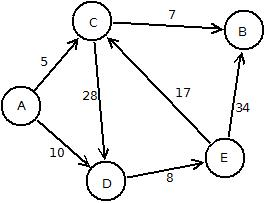
\includegraphics[scale=.7]{FIG1.jpeg}
\label{fig:1}
\end{figure}\\
From now on we can consider our problem as a routing problem.
We have a set of directed links $E$ representing the connections between the nodes and a set of \textit{source-destination} pairs $S$ where pair $(A,B)$ represents the agents wanting to travel from node $A$ to node $B$.\\
For each $s \in S$ we define $R(s)$ to be the set of routes connecting the \textit{source-destination} pair and $f(s)$ to be the amount of traffic on $s$. Moreover, we denote by $R$ the set of all the routes. Since for a given $s$ traffic from a source to a destination can be split into multiple routes, we define $x_r$ to be the amount of traffic of $s$ going through route $r$. Finally, we define $y_l$ to be the amount of traffic on link $l$ over all routes, i.e.~$y_l=\sum_{r | l \in r} x_r$.\\
On each link $l \in E$ there exists a delay which is a function of the traffic on that link, $y_l$, and is denoted $ D_l(y_l)$.  The delay function  is assumed to be convex, increasing and its first derivative to exist.\\\\
Thus the problem consists of minimizing the overall delay experienced by the agents.\\
To express the constraints of our optimization problem the following two matrices. \textcolor{red}{(Attention, this problem is not linear)}. Let $A$ be the link-route incidence matrix where $A_{lr}$ = 1 if link $l$ belongs to route $r$ and $A_{lr}$ = 0 otherwise. Secondly, let $H$ be the source-destination route incidence matrix where $H_{sr}$ = 1 if route $r$ connects $s$ and $H_{sr}$ = 0 otherwise.  Note that the summation of each column of $H$ is equal to 1, that means each route connects exactly one pair.\\\\
The optimization problem can be modelled as follows:
\begin{equation}
\begin{aligned}
& \underset{\x , \y }{\text{minimize}}
	& &  \sum_{l \in E} y_{l} D_{l}(y_{l}) \\
& \text{subject to}
      & &  y_{l} = \sum_{r|l \in r} x_{r}, \text{  }\forall l \in E\\
&       & & f_{s} = \sum_{r|s(r) = s} x_{r}, \text{  }\forall s \in S\\
&      &&  x_{r} \geq 0 , \text{  }\forall r \in R\\
\end{aligned}
\label{e:prob}
\end{equation}
,where $s(r)$ returns the source-destination pair that the route $r$ connects.

\section{A first approach to the solution}

In order to minimize the total delay experienced by all drivers, we need to find the local policies that will be followed. In the previous lesson we observed how a simple local policy can lead to the optimal solution. In this section we illustrate, with a  simple example, how a local policy which may seem logical and trivial may lead to a ``bad'' solution.\\\\
\begin{figure}[h!]
\centering
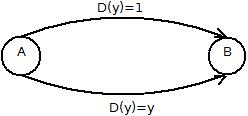
\includegraphics[scale=.7]{FIG2.jpg}
\label{fig:2}
\end{figure}\\
In our example, we have a flow of $1$ car per time unit between city $A$ to city $B$ and they can choose from two available routes. The upper route has a constant delay function of $D_{upper}=1$ and the lower has a linear delay function which is equal to the percentage of drivers that take that  route, $D_{lower} = y$.\\\\
The most natural approach would be for each driver to choose the route that has the lowest delay and in that way we expect all the drivers to face equal delay. \\
More formally, in the general case, we expect that $\forall r_1, r_2$ such that $s(r_1) = s(r_2), x_{r_1} > 0$ and $x_{r_2} > 0$ the delay will be $\sum_{l \in r_1} D(y_l) =  \sum_{l \in r_2} D(y_l) $.\\\\
Getting back to the example, the overall delay experienced  by drivers will be:
\begin{equation}
\label{e:TotDelay}
	 (1-\alpha) \times  D_{upper}(1-\alpha)  + \alpha \times  D_{lower}(\alpha) = (1-\alpha) \times 1 + \alpha \times \alpha,
\end{equation}

where $\alpha$ is the percentage of drivers that choose the lower route.\\
According to the aforementioned approach all drivers should choose the lower route as $D_{lower}$ would be lower than  $D_{upper}$. In this way $\alpha$ will be $1$ and the total delay will be $1$. But is this the optimal solution? \\
Minimizing the equation \eqref{e:TotDelay}  results to $\alpha^*=\frac{1}{2}$ and an overall experienced delay of $\frac{3}{4}= 0,75$. 



\section{Solving Problem~\eqref{e:prob} by the Lagrange multipliers method}

We can observe that the objective function of our optimization problem \eqref{e:prob} is convex. Indeed:
\begin{equation}
f(x) = y_l D(y_l) \Rightarrow f'(x) = y_l D'(y_l) + D(y_l) \Rightarrow f''(x) = y_l D''(y_l) + D'(y_l) + D'(y_l)
\end{equation}
$D''(y_l)$ and $ D'(y_l)$ are greater or equal to zero, for the hypotesis that $ D(y_l)$ is convex. So every terms in $f''(x)$ is non negative and thus the objective function is convex.\\
Another observation that we make is that each constraint is linear and that they define a set which is compact. Indeed, each variable $x_r$ is bounded:
\begin{equation}
0 \leq x_r \leq \underset{s \in S}{\text{max}} {f_s} \;\; \forall r \in R
\end{equation}
so the set set defined is closed and bounded.\\\\
Considering the previous observations we can apply the \emph{lagrange multipliers method} to apply theorem $(1)$ from the lesson 2. We define two set of multipliers:
\begin{enumerate}
\item one for each source-destination pair, $\lambda_s$, $ \forall s \in S$ and
\item one for each link, $\mu_l$, $\forall l \in E$.
\end{enumerate}
We can claim that  $\z^* = {\x^* \choose \y^*}$ is a global minimum for this optimization problem if and only if there exist $\lambda_s^*$, $\forall s \in S$ and $\mu_l^*$, $\forall l \in E$ such that:
\begin{enumerate}
\item $\x^*$ and $\y^*$ are feasible,
\item $\nabla_\x L(\z^*,\blambda^*,\bmu^*)^T (\z - \z^*) \ge 0,  \;\; \forall \z \in \{{\x \choose \y} ,\; \x \ge 0  \}$.
\end{enumerate}
The Lagrangian function results:
\begin{equation} 
L(z,\lambda,\mu)= \sum_{l \in E}  y_l D(y_l) + \sum_{s \in S} \lambda_{s} \left(f_s - \sum_{r:s(r)=s} x_r\right) + \sum_{l \in E} \mu_l \left(\sum_{r:l \in r} x_r - y_l\right) 
\end{equation}
When we differentiate it, we obtain:
\begin{equation}
\begin{aligned}
\frac{\partial L}{\partial y_l}=D(y_l)+  y_l D'(y_l) -  \mu_l  &&&&& &&&&& \frac{\partial L}{\partial x_r}=- \lambda_{s(r)} + \sum_{l \in r} \mu_l
\end{aligned}
\end{equation}
At the optimum, we have \textcolor{red}{(explanation missing)}:
\begin{equation}
\lambda^*_s(r)
\begin{cases}
= \sum_{l \in r} \mu^*_l & \mbox{if } x_r > 0,\\
\leq \sum_{l \in r} \mu^*_l & \mbox{if } x_r = 0,
\end{cases}
\end{equation}
and the quantity $\mu_l$ results:
\begin{equation}
\mu^*_l = D(y_l)+  y_l D'(y_l).
\end{equation} 
We can interpret the result for the multiplier $\mu_l$ like the cost that the drivers traversing link $l$ must pay. That cost is composed of the delay (i.e. $D(y_l)$) and the additional term $y_l D'(y_l)$. \textcolor{red}{(the interpretation of the additional term is missing)}. Furthermore, we can see $\lambda_{s(r)}$ the minimal cost available to source-destination pair $s(r)$.\\\\
With the previous observation, if we add tolls on the link, the drivers are encouraged to have a more desirable behaviour. Indeed we keep the example in the previous section and we add the toll $y_l D'(y_l)$ at the cost of each link. Each user experiences then two new costs for traveling the two paths. 
 $C_{upper}=1 + y_{upper} D'(y_{upper})= 1$ and   $C_{lower} = y_{lower} + y_{lower} D'(y_l)= 2y_{lower}$. Now the drivers choose the link where the total cost, delay plus toll, is minimum and the final solution is that half of the drivers choose the lower link and the others choose the upper link, that is the optimal solution for Problem \eqref{e:prob}.


%%%%  Bibliography goes here

\begin{thebibliography}{alpha}

\bibitem{Kel14} Frank Kelly and Elena Yudovina,
\newblock Stochastic Networks.
\newblock {\em Cambridge Press}, 2014.

\end{thebibliography}



\end{document}